% Import Packages
\documentclass[12pt,a4paper]{article}
\usepackage[utf8]{inputenc}
\usepackage{amsmath,amsfonts,amssymb} %math related
\usepackage{fixltx2e} %text subscript
\usepackage{circuitikz} %circuit drawings
\usepackage{fancyhdr} %fancy headers
\pagestyle{fancy} %something to do with page layout
\usepackage{float} %control over positions of figures etc
\usepackage{gensymb} %more symbols
\usepackage{graphicx} %importing graphics
\usepackage{hyperref} %refrencing
\usepackage{lipsum} %lorium ipsum
\usepackage{relsize} %text changing sizes
\usepackage{tabularx} %table controls
\usepackage{tikz} %drawings
\usetikzlibrary{calc,patterns,angles,quotes} %tikz add on
%\usepackage{times} %times new roman font
\usepackage{titling} %fancy titles
\newcommand{\textsub}{\textsubscript}
% make command for \subtitle
\newcommand{\subtitle}[1]{%
  \posttitle{%
    \par\end{center}
    \begin{center}\large#1\end{center}
    \vskip0.4em}%
}


%Title Page
\title{WTFpga?}
\author{{Developed by Joe FitzPatrick} \\
		{FOSSified by Piotr Esden-Tempski and Clifford Wolf}\\
		{Presented by Josh Johnson}} 


%set margins
\usepackage[left=2.5cm,right=2.5cm,top=2.5cm,bottom=2.5cm,headheight=1cm]{geometry}
\fancyheadoffset{0cm}
\lhead{WTFpga?}
\chead{}
\rhead{}
\lfoot{}
\cfoot{}
\rfoot{\thepage}
\renewcommand{\headrulewidth}{0.4pt}

\begin{document}
%Title Page
\begin{titlingpage}
    \maketitle
\end{titlingpage}

\newpage

\section{Introduction}
Welcome to the workshop! This is a hands-on crash-course in Verilog and FPGAs in general. It is self-guided and self-paced. Josh is here to answer questions, not drone on with text-laden slides like usual.

While microcontrollers run code, FPGAs let you define wires that connect things together, as well as logic that continuously combines and manipulates the values carried by those wires. Verilog is a hardware description language
that lets you define how the FPGA should work. 

Because of this, FPGAs are well suited to timing-precise or massively-parallel tasks. If you need to repeatedly process a consistent amount of data with minimal delay, an FPGA would be a good choice. Signal and graphics processing problems, often done with GPUs if power and cost are no object, are often easy to parallelize and FPGAs allow you to widen your pipeline until you run out of resources. As your processing becomes more complicated, or your data becomes more variable, microcontrollers can become a
better solution.

The objective of this workshop is to do something cool with FPGAs in only two hours. In order to introduce such a huge topic in such a short time, LOTS of details will be glossed over. Two hours from now you’re likely to have more questions about FPGAs than when you started - but at least you’ll know the important questions to ask if you choose to learn more.

\section{What We Won't Learn}
In order to introduce Verilog and FPGAs in such a short time, we’re going to skip over several things that will be important when you build your own FPGA-based designs, but are not necessary to kickstart your tinkering: 
\begin{itemize}
	\item Synchronous Logic: We’re dealing entirely with human (AKA slow) input and output today. Running at maximum performance requires synchronizing all of the logic using a common clock, and optimizing the logic to fit that enforced timing.
	\item IP Cores​: FPGA vendors pre-build or automatically generate code to let you easily interface your FPGA to interfaces like RAM, network, or PCIe. We’ll stick to LEDs and switches today.
	\item Simulation​: Didn’t work right the first time? Simulation lets you look at all the signals in your design without having to use hardware or potentially expensive observation equipment.
	\item Testbenches​: For effective simulation, you need to write even more Verilog code to stimulate the inputs to your system.
\end{itemize}

\newpage
\section{Meet the Hardware}
We will be using the not creatively named iCE40-feather board for this workshop. It contains an iCE40UP5K FPGA, USB programmer and USB to UART converter, LiPo battery charge control, and plenty of LEDs in an Adafruit Feather compatible form factor. To extend its capabilities for this workshop, we will be attaching a FeatherWing which has a dual seven segment display, and eight DIP switches. 

\begin{figure}[H]
\begin{centering}
	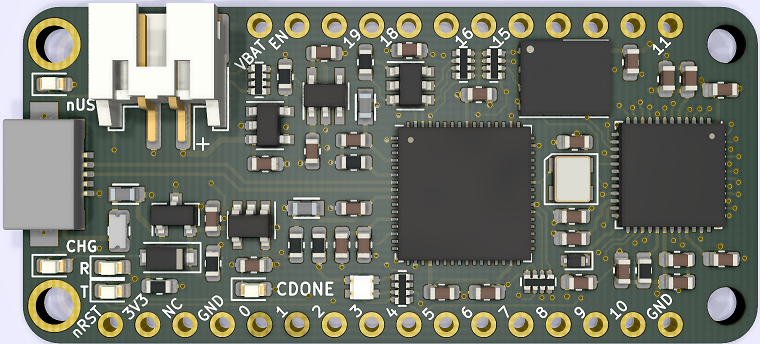
\includegraphics[width=\linewidth]{top_render.png}
	\caption{The iCE40-feather FPGA board being utilised.}
\end{centering}
\end{figure}

\begin{figure}[H]
\begin{centering}
	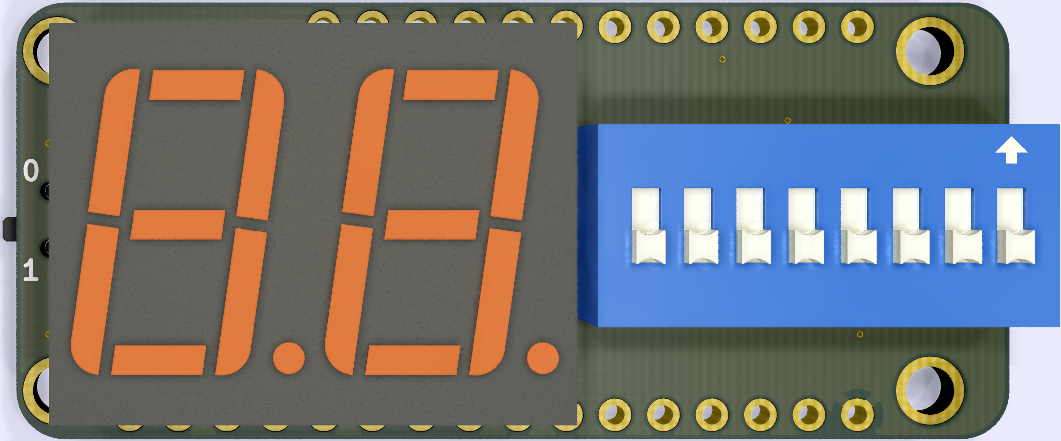
\includegraphics[width=\linewidth]{7segment_render.png}
	\caption{The seven segment and DIP switch FeatherWing.}
\end{centering}
\end{figure}
\newpage
\section{Getting to Blinky}
Due to time constraints, it is suggested that you install the toolchain and get a blinking LED on your iCE40-feather before attending the workshop. If you have not already installed the required Yosys, NextPNR, and IceStorm tools, follow the instructions in \texttt{install.md}. If you do not have the FPGA dev board, read the instructions in \texttt{README.md} and get in contact with Josh. \\

\noindent
With the toolchain installed and hardware in hand, it is now time to blink some LEDs! If you have not already done so, clone the repository and open the blink directory.\\

\noindent
\textbf{git clone https://github.com/joshajohnson/WTFpga} \\
\textbf{cd WTFpga/blink}\\

\noindent
Now its time to walk through the process of synthesizing an FPGA design of your own and uploading it to the FPGA. We will be using the amazing open source tools called IceStorm, NextPNR and Yosys. 
\begin{itemize}
		\item Ensure that the FPGA is connected via a USB cable to your computer. 
		\item Open the command line in the \texttt{WTFpga/blink} folder.
		\item Build and upload the gateware by typing \textbf{make prog} into the terminal. 
		\item Ensure that the led marked nUSR is blinking. If not it's time to begin troubleshooting!
		\item Once you get the LED blinking, open the file \texttt{blink.v} and have a look around. See if you can change the frequency of the blinking LED by altering the code. 
		\item After changing \texttt{blink.v} and saving it, run \textbf{make prog} again and confirm the frequency changes. 
\end{itemize}
If you have made it this far, congratulations! You have successfully programmed your FPGA, and can now attend the WTFpga workshop knowing that you'll hit the ground running. If you are having issues programming the board, get in contact with Josh and he will lend a hand troubleshooting. 
\end{document}
